\section{问题三：通信约束下的运输与中继联合调度}

题面把「连续通信」与货箱时限、载荷与能量、资源可用性并列为\textbf{约束}，即运输无人机在爬升、巡航、下降与投送的全过程都必须保持与调度中心的可通信状态。问题二的调度只优化了运输本身，沿其轨迹逐时刻判定直连链路可得如下事实：\textbf{71.67\% 的时间可直连，其余 28.33\% 处于通信盲区}。也就是说，若把中继保障作为事后补救，问题二的方案在通信连续性上根本不可行。本节把运输开始时刻、中继站选址与悬停高度、中继架次调度纳入同一个联合优化模型，并以“集合覆盖整数规划选站＋沿资源链级联错峰＋就绪性修复环”分层求解。

\subsection{联合优化模型}

\textbf{决策变量}（三层）：
\begin{itemize}
	\item 运输层：延续问题二的货箱组批与路线，把架次 $p$ 的开始时刻 $s_p$ 升为决策变量（即错峰量 $\Delta_p=s_p-s_p^{0}$）；
	\item 通信层：悬停站选址二元变量 $y_r\in\{0,1\}$，候选点 $r=(\lambda_r,\varphi_r,h_r)$ 同时含水平坐标与悬停离地高度 $h_r\in\{50,100,150,200,250,300\}$\,m；
	\item 调度层：中继架次的派发顺序与各架次的起飞、建链、服务、返航时刻。
\end{itemize}

\textbf{约束}：① 通信连续性 $C_p(t)=1,\ \forall p,\forall t$；② 问题二的全部约束在错峰后仍须成立（货箱硬时限、载质量与体积、返航能量余量、无人机与共享电池周转）；③ 中继侧的中继无人机与能源组件周转；④ 建链完成时刻不得晚于所服务失效区间的结束时刻。

\textbf{目标}为两层字典序：先\textbf{最小化通信中断时间}（须为 0），再在中断为 0 的前提下最小化悬停站数与中继总能耗。把「连续通信」写成必须归零的硬指标而非加权项，是因为题面已把它列为约束——加权只会把它降格为可交易项。

\subsection{直连失效区间与通信盲区}

对问题二推荐方案的每个运输架次，沿其三维轨迹（爬升、巡航、悬停交接、下降）按 $\Delta t$ 采样，逐点按式~\eqref{eq:pathloss} 计算路径损耗，并按第 \ref{sec:link-model} 节的双向链路门限判据判定直连可用性（含地形遮挡）。判定的一个有用性质是：\textbf{直连可用性只取决于轨迹的几何形状，与绝对时刻无关}，故错峰平移不会改变直连时间占比——这也是后文三组对照中直连占比恒为 $71.67\%$ 的原因。

在联合优化后的排班上，24 个运输架次中共有 19 个出现连续失效，形成 \textbf{19 个失效区间}（编号 G01--G19，逐区间明细见 \texttt{q3\_intervals.csv}），其时间之和占全部飞行时间的 $28.33\%$。区间在空间上分为若干片互不相连的地形阴影区，需由不同位置的悬停站分别覆盖，如图~\ref{fig:q3-relay}中的红色散点所示。

\begin{figure}[htbp]
	\centering
	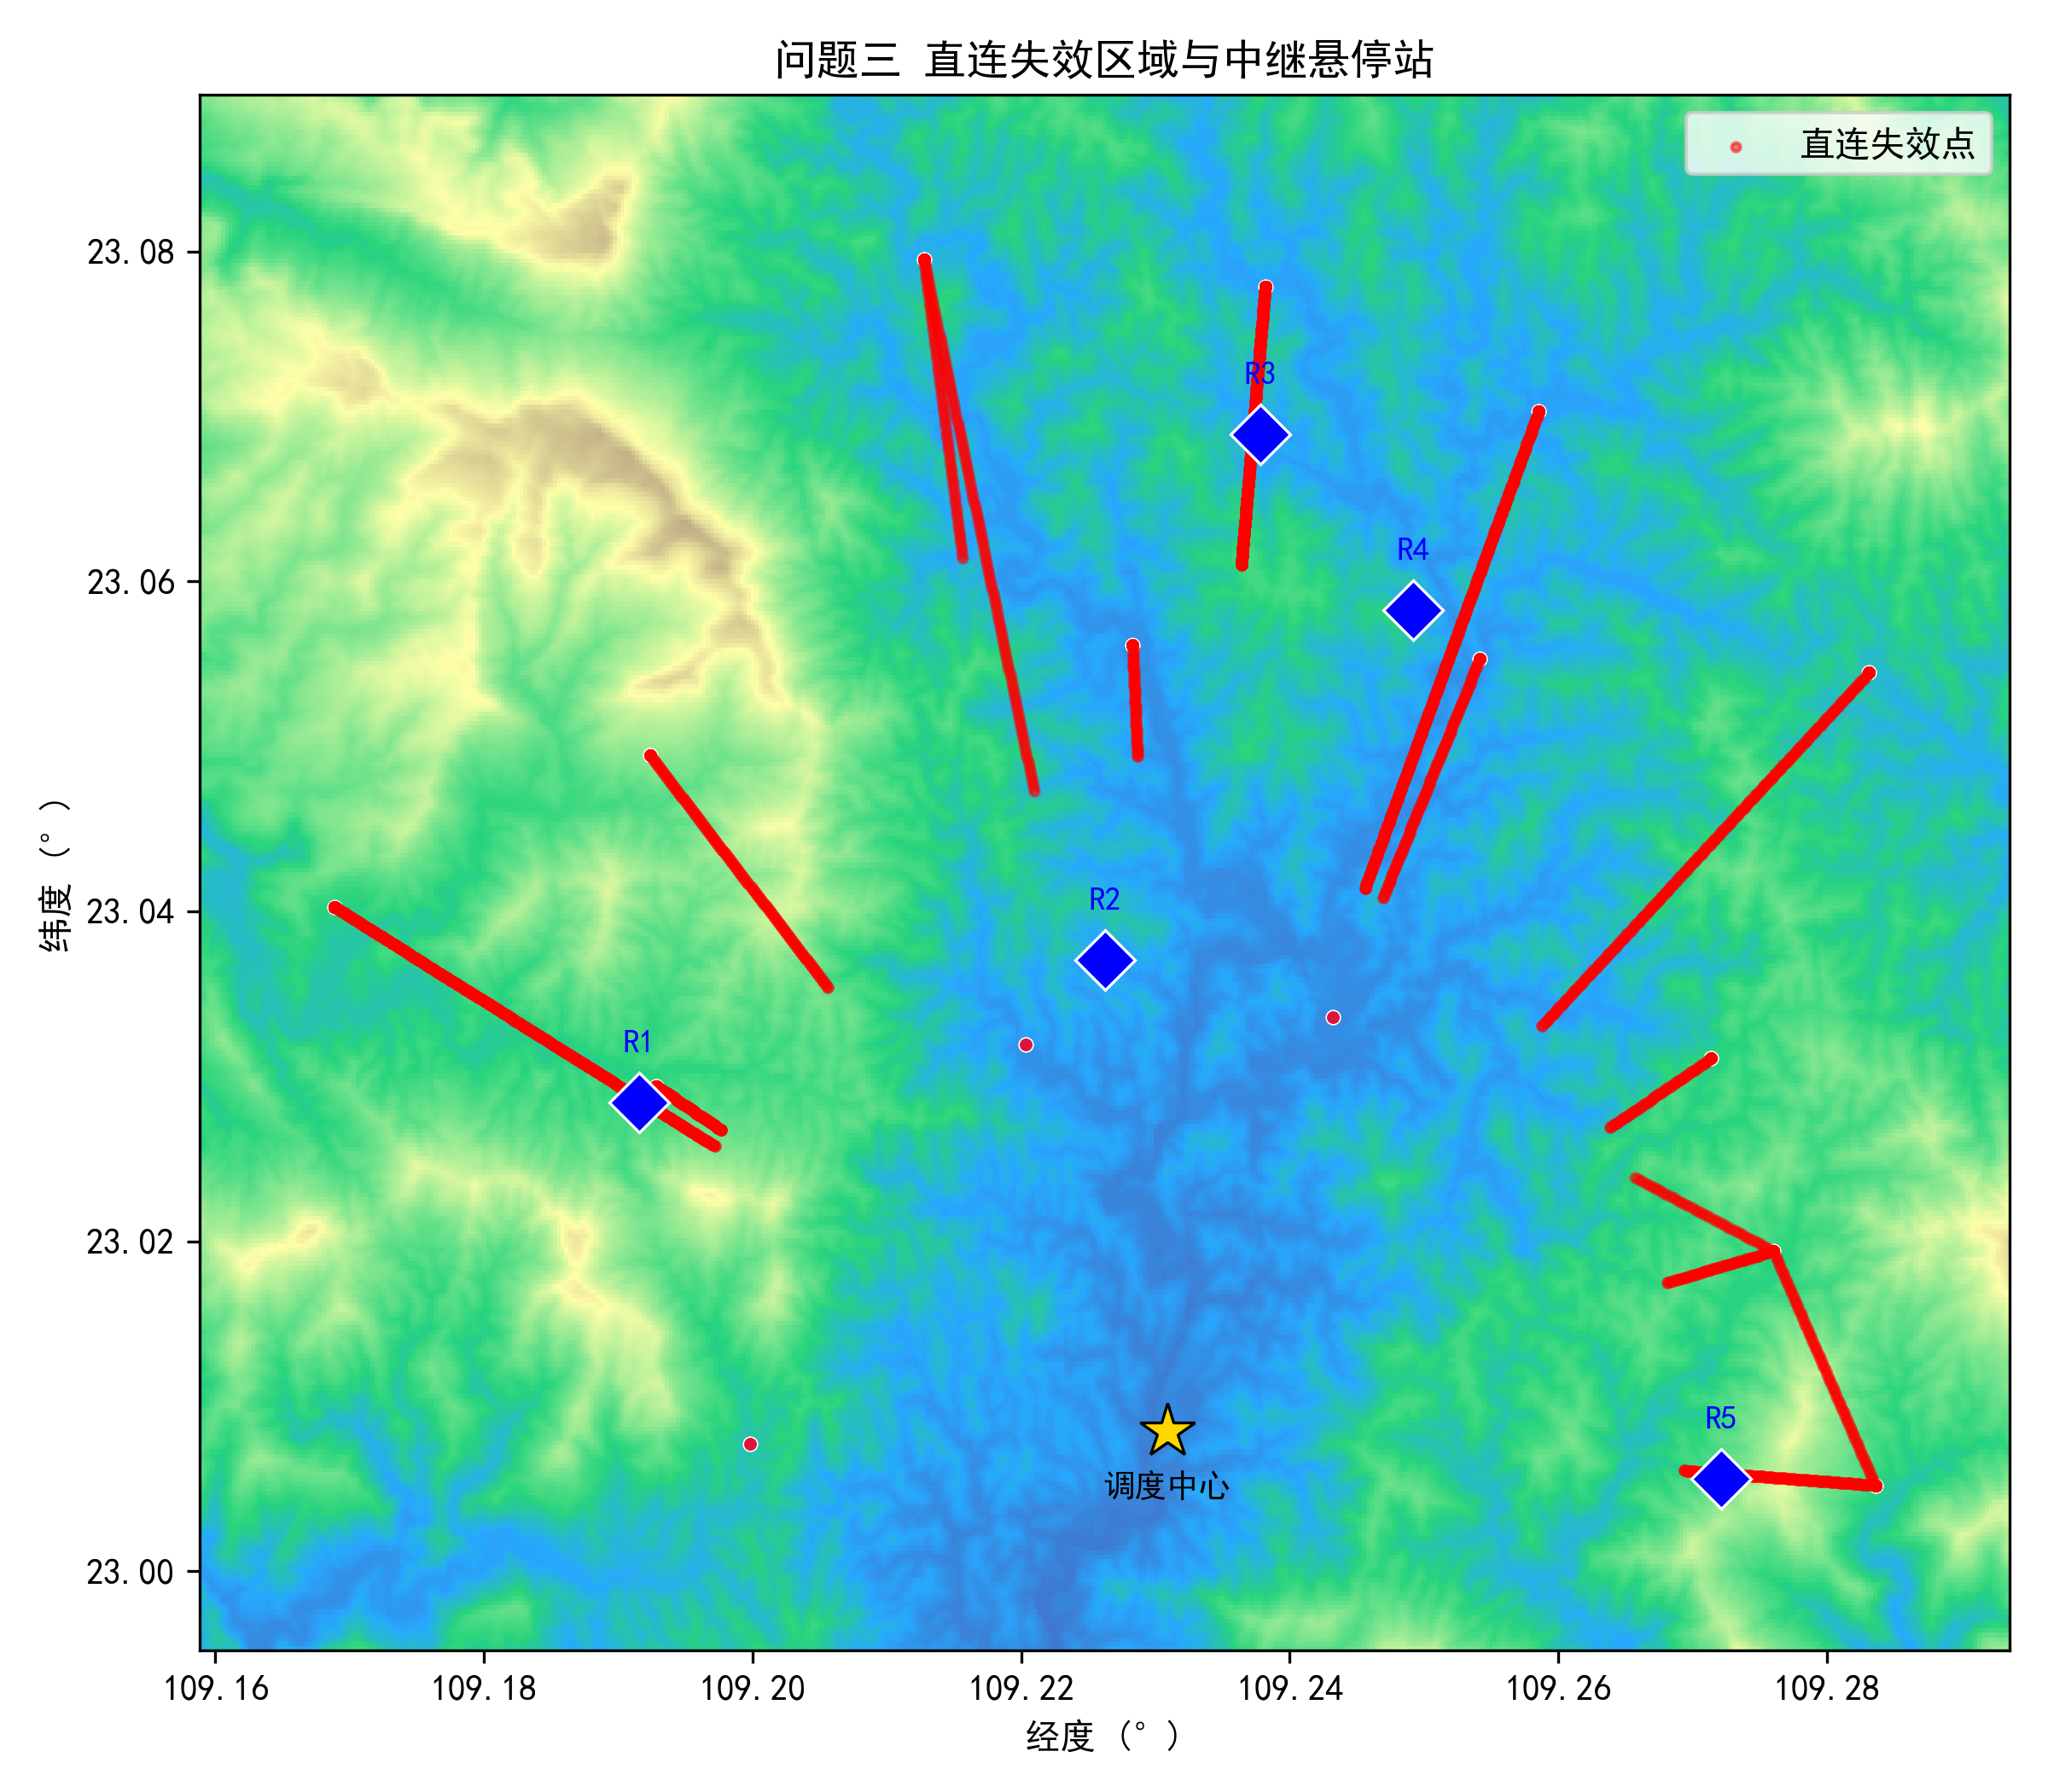
\includegraphics[width=0.82\textwidth]{figures/fig_q3_relay.png}
	\caption{直连失效区域与中继悬停站}
	\label{fig:q3-relay}
\end{figure}

\subsection{三维悬停站的集合覆盖选址}

候选悬停点由失效点包围盒内步长 1200\,m 的水平网格（$11\times8$）与 6 档离地高度交叉生成\cite{elnabty2022survey}，共 \textbf{342 个}，保留其中能与 G01 建立回传链路者。对候选点 $r$ 与失效区间 $j$ 预计算覆盖系数 $a_{jr}\in\{0,1\}$：$a_{jr}=1$ 当且仅当 $r$ 在 $h_r$ 高度上能对区间 $j$ 所属运输架次的\textbf{全部}轨迹采样点建立接入链路。本算例每个区间的可覆盖站数为 22--204 个，不存在无站可覆盖的区间。选站即求解集合覆盖问题\cite{church1976theoretical}
\begin{equation}
	\min \sum_{r} y_r \quad \text{s.t.}\quad \sum_{r} a_{jr}\,y_r \ge 1,\ \ \forall j,
	\label{eq:setcover}
\end{equation}
再以两层字典序求解：先最小化站数，再在最小站数下最小化中继总能耗。求解过程中先以粗步长（每 5 个采样点取 1）构造覆盖矩阵以免假负例，随后对入选的 $(j,r)$ 对做\textbf{全密度复核}，剔除实际覆盖不完全的列并重解，构成列生成式的修复环。最后用坐标下降法对 $({\rm lon},{\rm lat},h)$ 做连续局部微调，最大化该站对最不利采样点的接入裕量。

集合覆盖先给出 \textbf{3 个悬停站}，几何上已覆盖全部 19 个区间。但「几何上覆盖」不等于「届时守得住」：中继机只有 2 架，某些区间在其被覆盖的站上等不到中继机到位。第 \ref{sec:q3-repair} 节的\textbf{换站修复}为此改换部分区间的归属站，另引入 2 个站，最终方案共 \textbf{5 个悬停站}（表~\ref{tab:q3-stations}）。

\begin{table}[htbp]
	\caption{中继悬停站选址结果}
	\label{tab:q3-stations}
	\centering
	\small
	\begin{tabular}{cccccc}
		\toprule
		编号 & 经度（$^\circ$） & 纬度（$^\circ$） & 地面高程（m） & 离地高度（m） & 保障区间数 \\
		\midrule
		S01 & 109.1916 & 23.0284 & 359.03 & 100 & 5 \\
		S02 & 109.2262 & 23.0371 & 211.09 & 300 & 3 \\
		S03 & 109.2378 & 23.0689 & 245.42 & 200 & 4 \\
		S04 & 109.2492 & 23.0583 & 252.18 & 300 & 1 \\
		S05 & 109.2721 & 23.0056 & 407.44 & 190 & 6 \\
		\bottomrule
	\end{tabular}
\end{table}

值得注意的是，五站的离地高度为 $100$、$300$、$200$、$300$、$190$\,m：\textbf{三站落在中间档、两站顶到题给上限 $300$\,m}。这说明悬停高度是一个真正起作用的决策变量，但它的作用是\textbf{非单调}的——选站的字典序目标是最小化站数、再最小化中继总能耗，而站址与离地高度的连续精化准则是最大化该站对所辖区间最不利采样点的接入裕量（同时保持回传可用、不超高度上限）。当地形阴影较深时，抬高到上限是唯一能建立接入的选择；当阴影较浅时，中间档即可满足裕量，无须付出额外爬升。故不能笼统地说「最优解不会顶到上限」，只能说\textbf{是否顶到上限由该片阴影区的地形决定}。

\subsection{中继架次调度与运输错峰}
\label{sec:q3-repair}

\textbf{服务时段合并。}一个悬停站在一段时间内往往要连续保障多个运输架次的失效区间，若逐段派发会产生大量固定开销（起飞准备、爬升建链、返航周转）。故\textbf{只按悬停站分组}，把同一站上间隔不超过 $900$\,s 的失效区间合并为一个中继服务任务，并限制单个任务跨度不超过 $3600$\,s；合并\textbf{不要求这些区间来自同一运输架次}，因为中继机在合并窗口内持续悬停，与它此刻保障的是哪一架运输机无关，跨架次合并正是省下整次出动的主要来源。本算例的 19 段失效区间经合并后只需 7 次悬停服务。

\textbf{中继架次能耗。}每个中继架次 $k$ 的能耗按题给口径由水平巡航、爬升附加与悬停通信三部分组成：
\begin{equation}
	E^{R}_{k}=P^{c}_{R}\frac{d_{k}}{v^{c}_{R}}\frac{1}{3600}
	+\frac{1}{3.6\times10^{6}}\cdot\frac{m^{\mathrm{TO}}_{R}\,g\,h^{+}_{k}}{\eta^{\uparrow}_{R}}
	+\big(P^{\mathrm{hover}}_{R}+P^{\mathrm{comm}}_{R}\big)\frac{t^{\mathrm{svc}}_{k}}{3600},
	\label{eq:relay-energy}
\end{equation}
其中 $m^{\mathrm{TO}}_{R}$ 为计划起飞总质量（悬停与爬升均按此质量计），$t^{\mathrm{svc}}_{k}$ 为悬停服务时长；三项分别由 kW$\cdot$s 与 J 折算为 kWh 后求和。每个中继架次同样须满足返航电量约束 $E^{R}_{k}\le(1-\rho_{R})E^{\mathrm{use}}_{R}$。

\textbf{弃飞规则。}若某中继架次飞抵悬停点并完成建链的时刻已晚于所服务失效区间的结束时刻，则该架次提供不了任何通信保障。这类架次不能「照飞不误」——它同样占用一架中继无人机和一组能源组件，会把后续本可按时到达的架次一并顶迟到，形成级联迟到。故调度规则中显式加入一条：\textbf{建链时刻晚于区间结束时放弃派发该架次}，弃飞数在结果中如实报告。

\textbf{运输错峰。}在保持问题二组批与路线不变的前提下，把各运输架次的开始时刻后移，使同一时刻需要中继保障的\textbf{不同悬停站}数不超过 2（题给的中继无人机数）。错峰不是简单的削峰：单个架次的后移会被同一条无人机/电池资源链上的下一架次顶回，因此本文沿资源链\textbf{级联传播}推迟量，而非逐架次试探。其后还有两级修复：\textbf{就绪性修复}把「中继届时尚未到位」的区间所属运输架次沿资源链后移，直到中继建链完成时刻不晚于区间起点（推迟上限受货箱硬时限的松弛量约束）；\textbf{换站修复}则在就绪性修复已顶死硬时限时，把区间改派给「中继届时真在位」的另一个站，补上集合覆盖看不见的时间维度。实测就绪性修复是推迟量的主要来源：最终 11 个被推迟架次中，多数架次的失效区间起点\textbf{恰好等于}其所绑中继架次的建链完成时刻（例如 T17 的 G12 起点 $8265.2$\,s 即 R06 的建链完成时刻、T23 的 G18 起点 $8575.6$\,s 即 R07 的建链完成时刻），说明这些架次的开始时刻是被中继链的到位时刻反推锁定的，而不是搜索取大的结果。

\subsection{问题二最优解的等价类：用第三问门禁择序}
\label{sec:q2-gate}

上述修复环解决的是「中继到位与运输到达的时序错配」。实施中还暴露出一个更靠上游的问题，本文如实记录并给出处置。

问题二的目标是「加权时延 $\to$ 完工时刻 $\to$ 能耗 $\to$ 架次数」的字典序，其中前两项与\textbf{每架无人机的总占用时长}有关，而与「同一架无人机上两个架次谁先飞」无关——调换先后不改变该机的总忙碌时间，故问题二的\textbf{最优解是一个等价类}，类内各元素的架次数、完工、能耗、加权时延可以逐位相同。但第三问的通信保障依赖\textbf{绝对时刻}：某个架次的失效区间若落在中继链的尾端，中继机返航周转赶不上，就会出现几百秒的迟建链。原方案正是如此：\textbf{195 个采样点（占全部时间的 $0.6688\%$）无人保障}，且这一缺口无法靠第三问单独消去——因为第三问只被允许改变各架次的开始时刻，而问题二的下游校验要求 \texttt{q3\_stagger.csv} 的「原开始时刻」恒等于问题二架次表的「开始时刻」（见第 \ref{sec:q3-check} 节），顺序必须由问题二本身给出。

故本文在问题二内部增加一层\textbf{确定性门禁}（\texttt{q2\_v2.relay\_feasible\_order}）：按无人机编号升序、下标升序枚举「同机两架次互换」的全部候选（本算例 24 个架次共 25 个候选），只保留使 \texttt{q2.evaluate} 报告的五项指标（架次数、完工、能耗、加权时延、硬违反）\textbf{逐位相等}的候选（实测 3 个），再把这 3 个候选与原序一并交给第三问，按第三问的字典序（无绑定区间数 $\to$ 缺口秒数 $\to$ 累计推迟量 $\to$ 联合完工 $\to$ 中继能耗）择优选出一条。由此：

\begin{itemize}
	\item \textbf{论文中报告的问题二数字一个都不变}——该层只改「谁先飞」，不改任何指标（代码中以断言 \texttt{assert \_relay\_metric\_key(m2) == base\_key} 把关）；
	\item \textbf{结果可复现}——候选枚举与排序都是确定性的，同种子跑两遍得到同一个顺序；
	\item \textbf{基线与候选一同参与比较}，故门禁不会把一个已经更好的顺序换差。
\end{itemize}

门禁最终选中无人机 U06 上派发序列第 6 位与第 8 位互换。问题二的五项指标逐位不变，而第三问的中断由 $0.6688\%$（195 个采样点）\textbf{降为 0}。这是一次\textbf{有代价的交换}，代价在第 \ref{sec:q3-cost} 节如实报告。

\subsection{求解结果与对照}

联合优化后共派发 \textbf{7 个中继架次}（R01--R07），由 2 架中继无人机分别飞 3 趟与 4 趟（R01$\to$\allowbreak R04$\to$\allowbreak R07 与 R02$\to$\allowbreak R03$\to$\allowbreak R05$\to$\allowbreak R06），占用 6 组能源组件（RC2 周转两次），弃飞 0 架次、迟建链 0 架次、未保障区间 0 个，中继总能耗 \textbf{4.493\,kWh}。19 个失效区间与中继架次的绑定关系完整给出（表~\ref{tab:q3-bind}节选），每站的保障区间数与表~\ref{tab:q3-stations}一致。

\begin{table}[htbp]
	\caption{运输架次—失效区间—中继架次绑定（节选）}
	\label{tab:q3-bind}
	\centering
	\small
	\begin{tabular}{cccccc}
		\toprule
		区间 & 运输架次 & 区间起点（s） & 区间终点（s） & 悬停站 & 中继架次 \\
		\midrule
		G01 & T04 & 2533.4 & 3479.5 & S02 & R03 \\
		G02 & T05 & 706.8 & 1232.8 & S05 & R01 \\
		G03 & T06 & 813.1 & 1235.0 & S01 & R02 \\
		G12 & T17 & 8265.2 & 8854.9 & S04 & R06 \\
		G13 & T18 & 5297.9 & 5948.1 & S03 & R05 \\
		G18 & T23 & 8575.6 & 9193.6 & S03 & R07 \\
		\bottomrule
	\end{tabular}
\end{table}

\textbf{三组口径对照。}为把「联合优化究竟带来了什么」讲清楚，本文按同一套时间积分口径（$\Delta t=1$\,s）给出三组对照（表~\ref{tab:relay-gap}）：\emph{无中继}即问题二的纯运输调度，\emph{序贯对照}为固定悬停高度 $300$\,m、贪心选站、不错峰、不做高度选择与连续精化的常规做法，\emph{联合优化}即本节方案。

\begin{table}[htbp]
	\caption{三种通信保障口径的对照（$\Delta t=1$\,s 时间积分）}
	\label{tab:relay-gap}
	\centering
	\small
	\setlength{\tabcolsep}{4pt}
	\begin{tabular}{lccccc}
		\toprule
		口径 & 直连占比 & 中继占比 & \textbf{中断占比} & 中继架次 & 中继能耗（kWh） \\
		\midrule
		无中继（问题二调度） & 71.67\% & 0 & \textbf{28.33\%} & 0 & 0 \\
		序贯对照 & 71.67\% & 24.22\% & \textbf{4.11\%} & 3 & 3.019 \\
		\textbf{联合优化} & 71.67\% & 28.33\% & \textbf{0.00\%} & 7 & 4.493 \\
		\bottomrule
	\end{tabular}
\end{table}

可见三点。其一，\textbf{中继不是锦上添花而是必需}：不做中继时运输全过程有超过四分之一的时间处于通信盲区，方案在题面约束下不可行。其二，把高度、站址、错峰纳入决策后，中断由序贯方案的 $4.11\%$ 归零，付出了 4 个额外中继架次与 $1.47$\,kWh 的能耗——序贯对照之所以只需 3 架次，正是因为它\emph{不管}剩余 $4.11\%$ 的盲区，两者的架次数不能直接相比。其三，直连占比在三组中完全一致，说明所有改善都来自中继侧与错峰的协同，而不是通过改变航线「绕开」阴影区。

图~\ref{fig:q3-timeline}以时序带的形式给出结论：上方为每个运输架次的通信状态（直连/中继/中断三色），下方为 7 个中继架次的占位窗口；可以看到全部架次带中\textbf{不存在中断色段}，且任一时刻占位的中继架次不超过 2 个，与题给的 2 架中继无人机容量相符。

\begin{figure}[htbp]
	\centering
	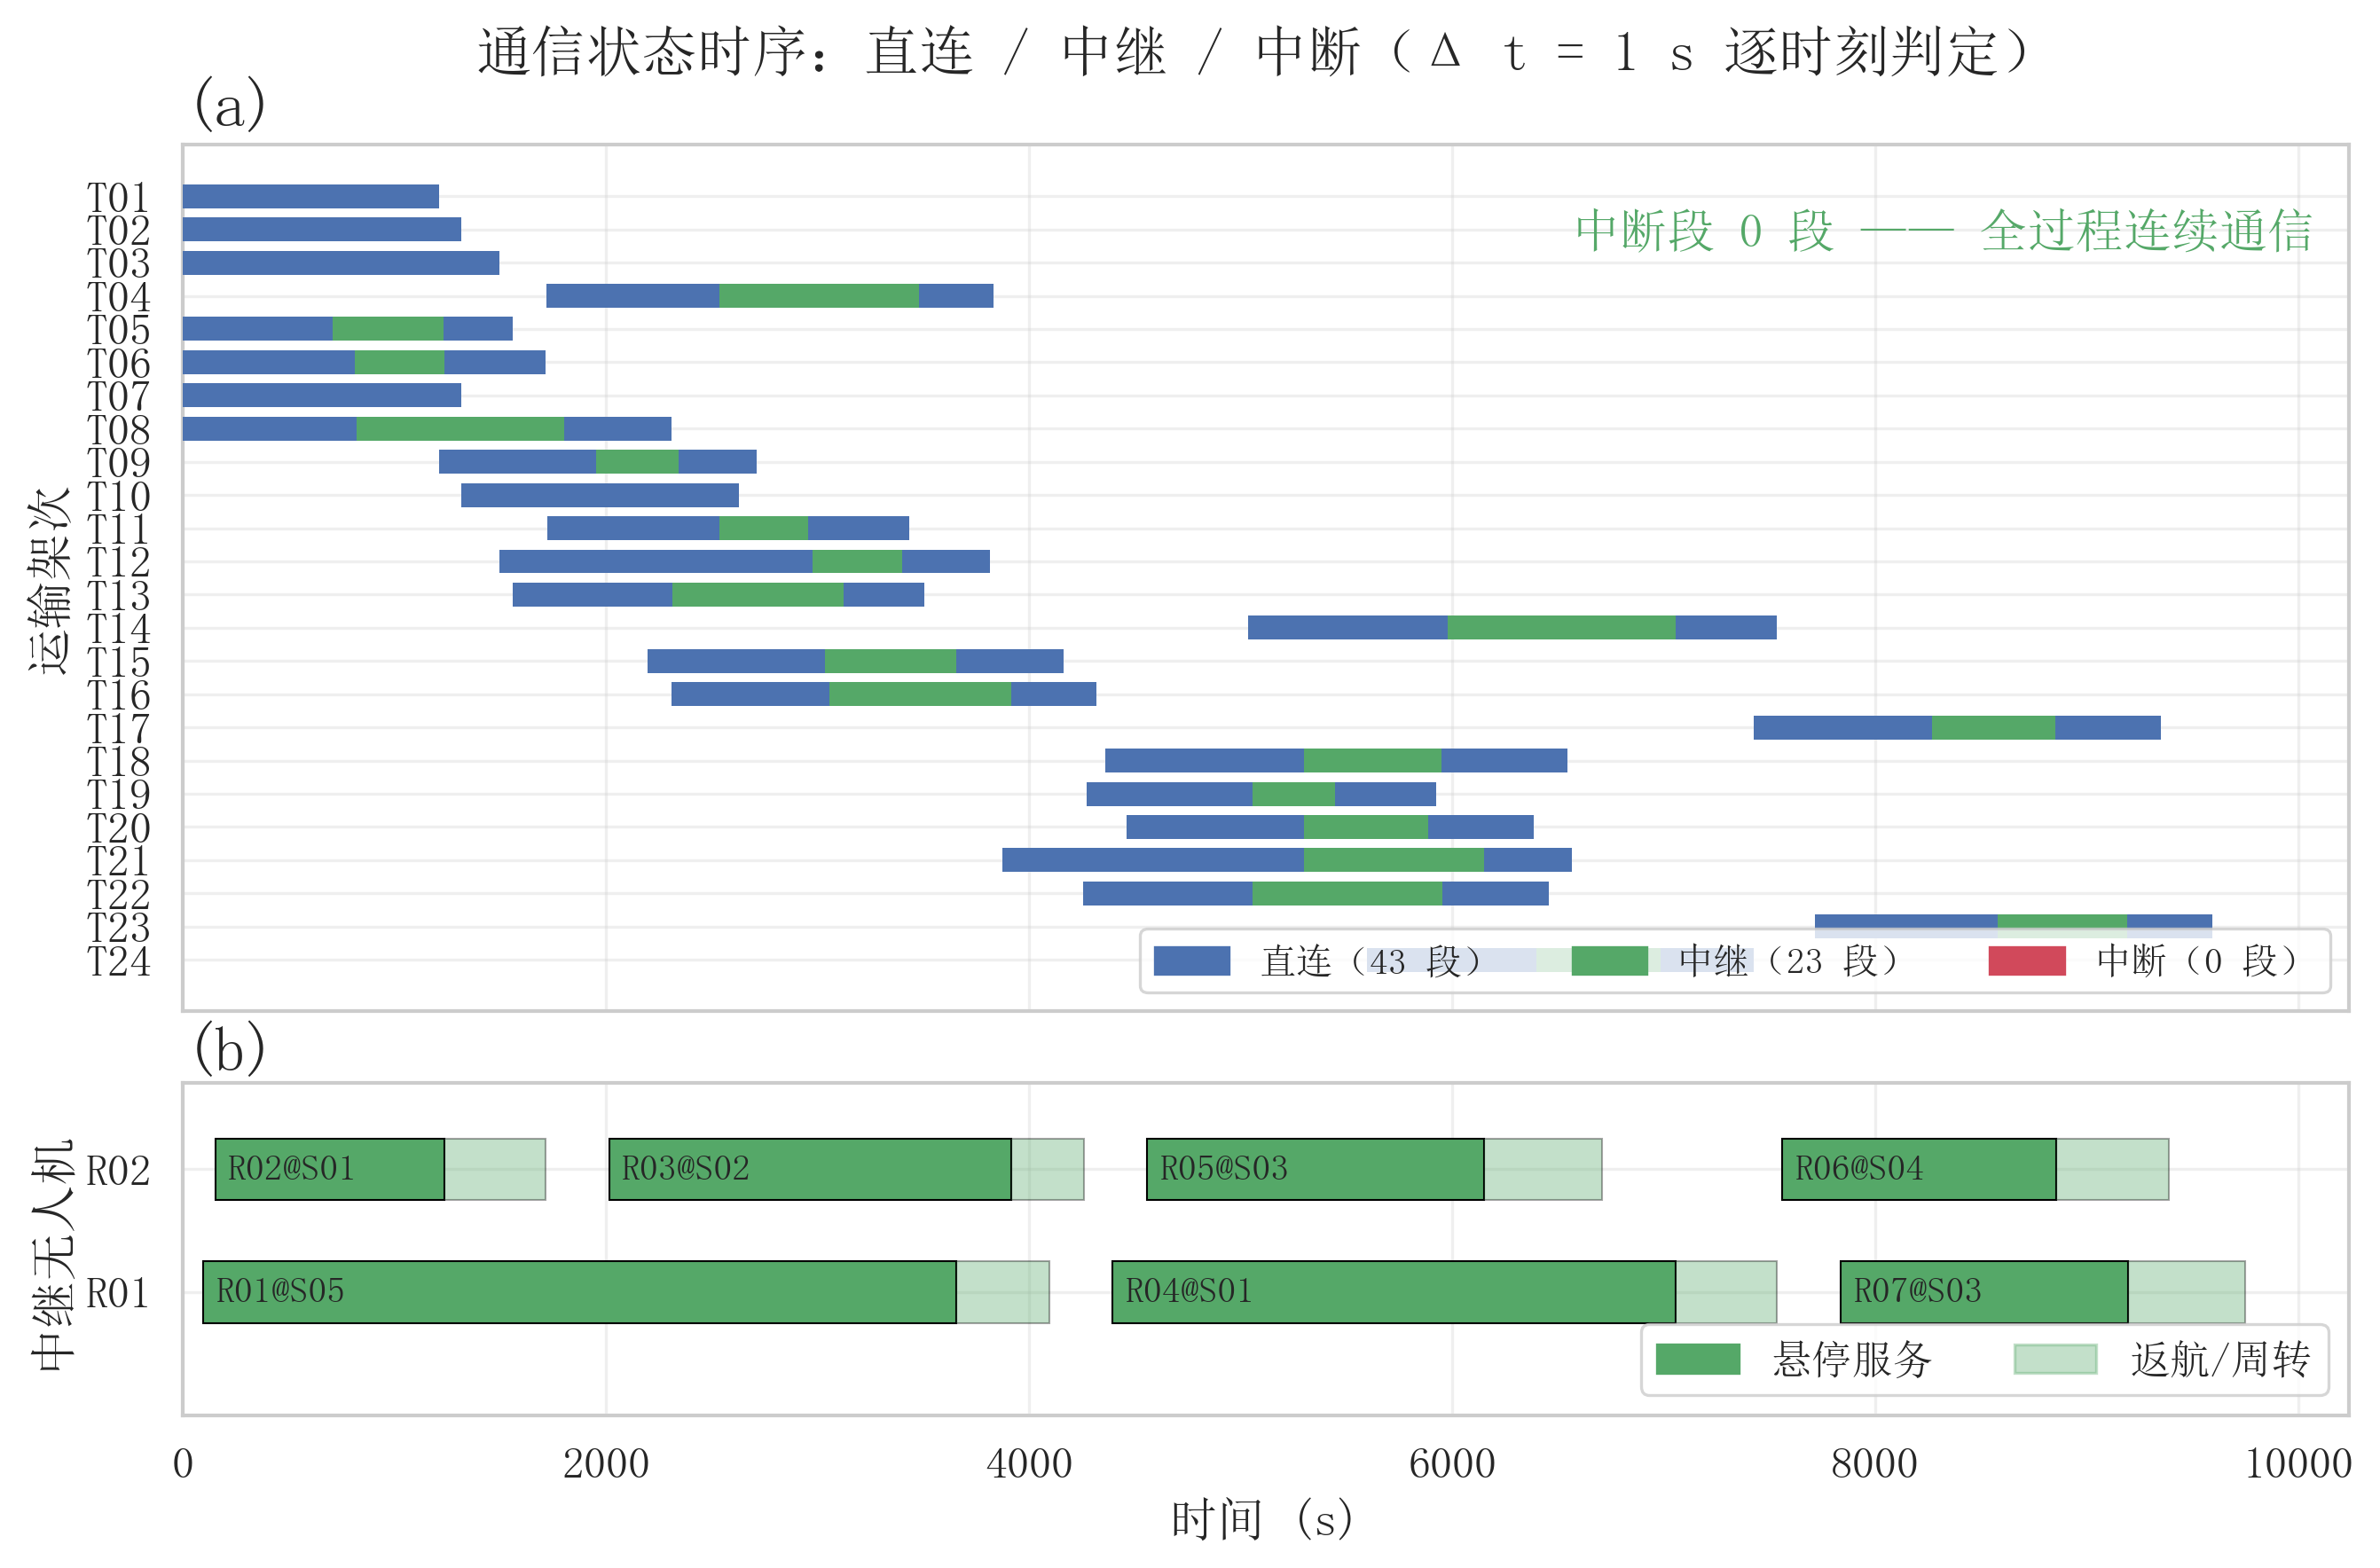
\includegraphics[width=0.95\textwidth]{figures/fig_q3_timeline.png}
	\caption{通信状态时序带与中继服务窗口}
	\label{fig:q3-timeline}
\end{figure}

图~\ref{fig:q3-analysis}给出中继侧的几何诊断：五个悬停站在地形上的三维位置、各站的接入裕量分布与覆盖区间数。五站中 S05 与 S01 承担的区间最多（6 个与 5 个），S03 覆盖 4 个，S02 覆盖 3 个，S04 只压住 1 个区间——S04 正是换站修复为 G12 单独引入的那个站，它印证了「几何覆盖」与「时序可达」是两件不同的事。

\begin{figure}[htbp]
	\centering
	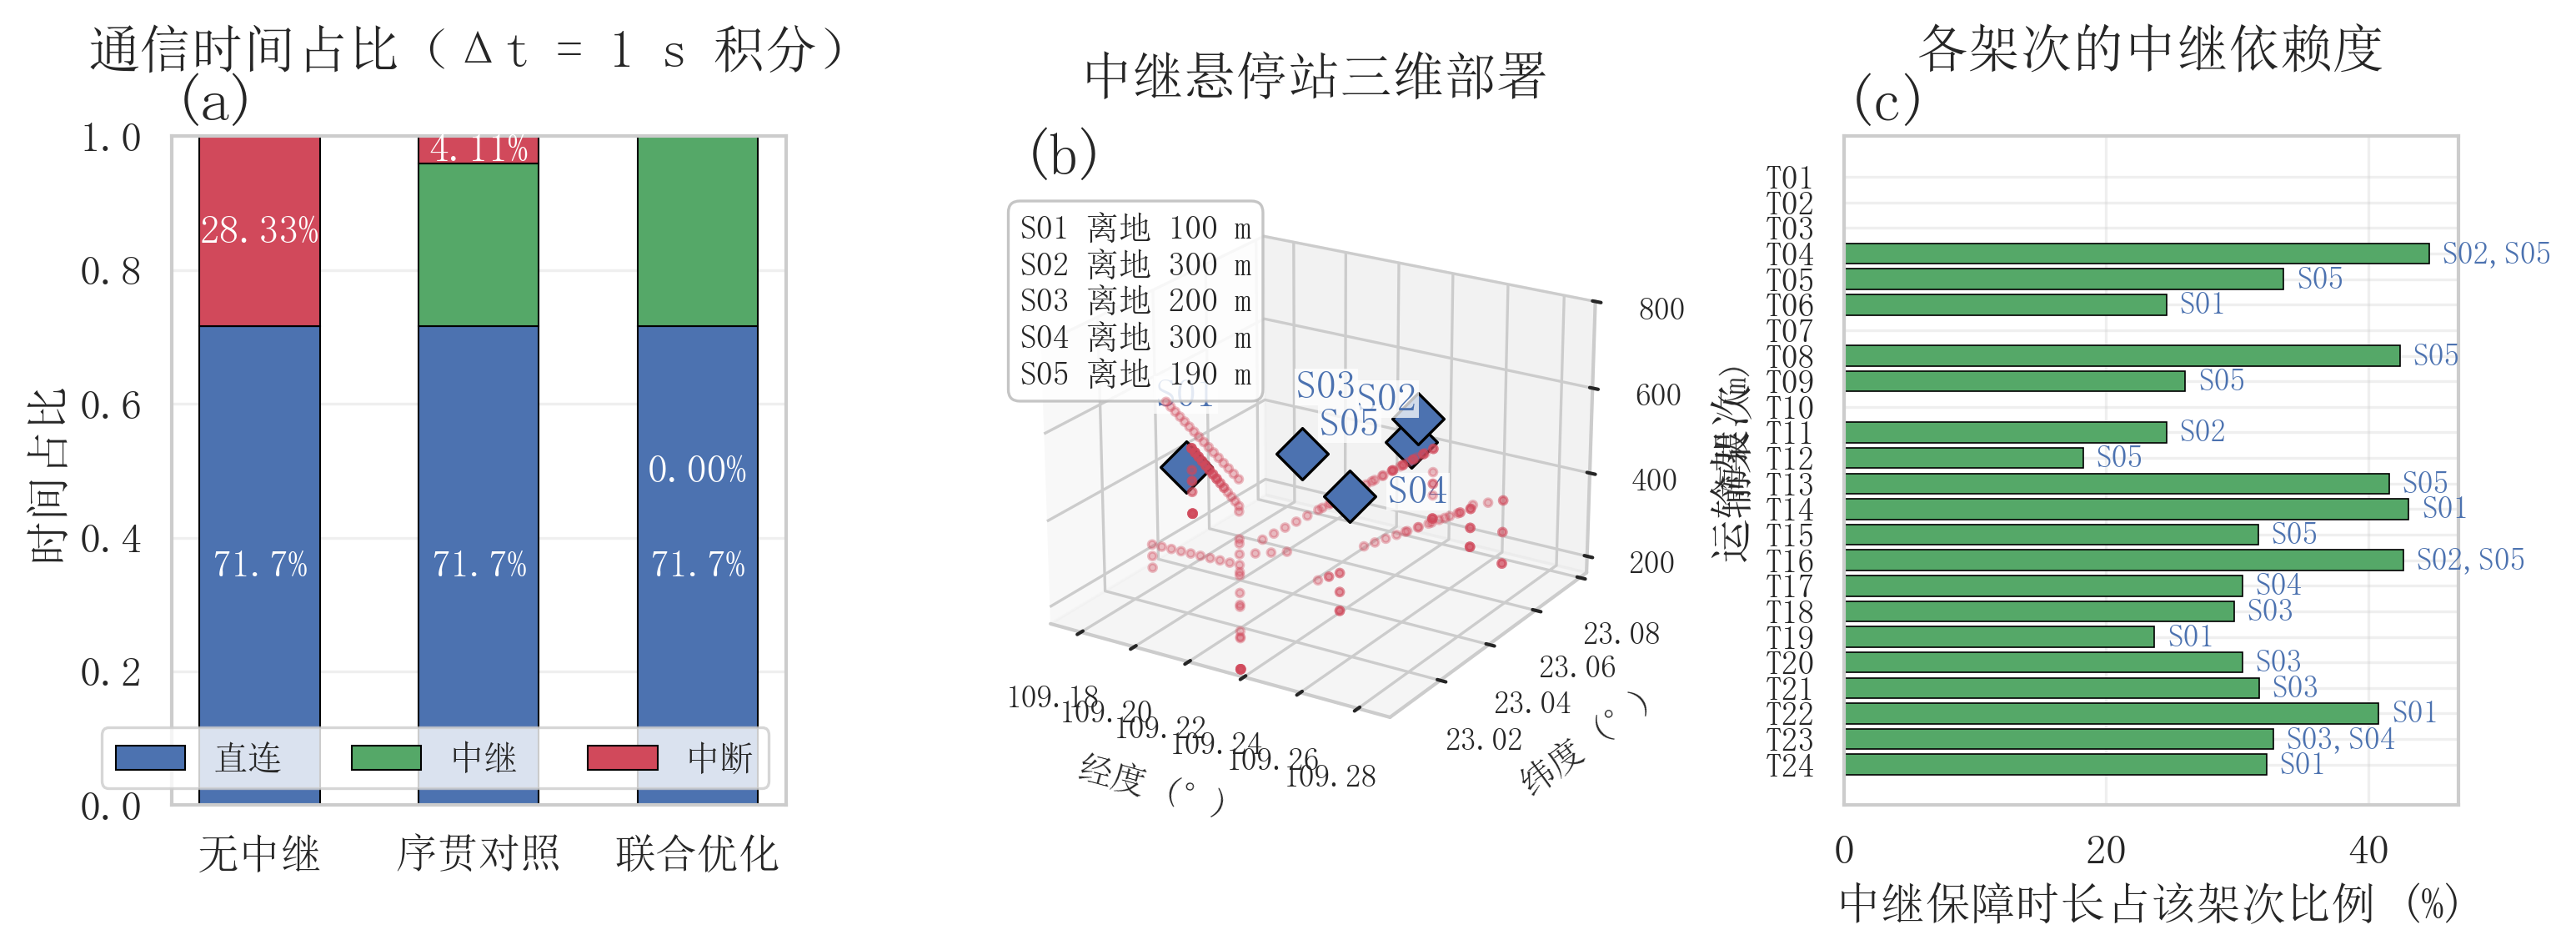
\includegraphics[width=0.95\textwidth]{figures/fig_q3_analysis.png}
	\caption{悬停站三维位置与链路裕量分布}
	\label{fig:q3-analysis}
\end{figure}

\textbf{一条未采用的并列路径（如实记录）。}本节另实现了一条「运输重排 $\leftrightarrow$ 中继归属」的固定点迭代错峰路径（\texttt{code/q3\_v2.py}），两条路径都跑完再按同一字典序择优，旧路径原地保留。实测该路径在 12 轮上限内\textbf{未收敛}：累计释放量逐轮单调增长（第 1 轮 $0$\,s $\to$ 第 12 轮 $33\,388$\,s），每轮都在把运输架次继续往后推而不进入不动点，其末端解的缺口仍有 $1694$\,s（对应 4 个失效区间无人保障），累计推迟达 $43\,342$\,s、加权迟到 $282\,463$、联合完工 $13\,108$\,s、中继能耗 $5.409$\,kWh，在字典序的每一层上都劣于现有方案。故\textbf{该路径本次未被采用}，择优判据与逐轮记录都留在运行日志中，未静默丢弃。本文据此指出：在这类「释放时刻随排班自增」的耦合问题上，固定点迭代并不自动收敛，把未收敛的迭代结果当作解使用会得到一个表面上「零弃飞」、实则留下大段盲区的方案。

\subsection{零中断的代价}
\label{sec:q3-cost}

通信连续性归零不是免费的，本文如实报告其代价。第一，\textbf{联合完工时刻由问题二的 $6506.1$\,s 推迟到 $9749.5$\,s，增加 $3243.4$\,s（$+49.9\%$）}；其中运输侧的完工由 $6506.1$\,s 推迟到 $9594.4$\,s（$+47.5\%$），其余 $155.1$\,s 是中继最晚返航造成的。第二，共有 \textbf{11 个运输架次被推迟，累计推迟 $17\,291.5$\,s}，推迟量最大的五个是 T17（$4714.5$\,s）、T23（$3097.3$\,s）、T14（$2918.3$\,s）、T04（$1718.2$\,s）、T18（$1598.4$\,s）。第三，交付侧出现 \textbf{1 个迟到货箱}（S004-WAT-03，由 T17 承运，比期望送达时刻晚 $1470.7$\,s，加权迟到合计 $14\,707.0$ 权重$\cdot$s）；该箱属饮用水、题面未给硬时限，故\textbf{货箱硬时限零违约仍然成立}，但全方案的最小硬时限余量已只剩 \textbf{$5.35$\,s}（S002-WAT-01）。第四，中继侧额外消耗 $4.493$\,kWh 与 6 组能源组件周转。

必须说明这四项代价与第 \ref{sec:q2-gate} 节的门禁之间的因果：门禁在第三问字典序里把\textbf{缺口秒数排在累计推迟量之前}，因此它选择了「用推迟换零中断」。这一排序不是任意设定的——题面把连续通信列为\textbf{约束}、把送达时刻列为\textbf{优化目标}（且饮用水只有期望时刻、没有硬时限），故先保证约束、再优化目标符合题目给出的层次。但代价是真实的：若把加权迟到置于缺口之前，原序方案（缺口 $0.6688\%$、加权迟到 $0$、累计推迟 $13\,481$\,s、中继 6 架次、$4.0457$\,kWh）会在该指标上更优，而它\textbf{在题面约束下不可行}。本文不给「两全」的假象，只报告这一取舍。

\subsection{口径说明}

本节的三组占比一律采用\textbf{时间积分口径}：以 $\Delta t=1$\,s 离散化，每点权重取 $w_i=(t_{i+1}-t_{i-1})/2$，再按状态累加，因此占比是时间占比而非采样点个数占比。这一改动是必要的：轨迹在爬升、巡航、悬停交接各段的采样密度并不相同，按点数统计会系统性偏向采样更密的阶段。此外，判定中继覆盖时须同时满足「该悬停站此刻确实能连通这架运输机」与「该中继架次此刻已完成建链且尚未结束服务」，而不能只检查时刻是否落在某个在役中继的时间窗内——后者会把「站在服务、但几何上够不着」的时段误记为已覆盖，从而虚高中继覆盖率。本文的早期版本正是采用了后一种粗口径，故其报出的覆盖率偏高、中断率偏低，最终结论以本节的逐点判定为准。

\textbf{运输侧的飞行高度不在决策空间内。}表~\ref{tab:relay-gap} 中直连占比在三组口径下恒为 $71.67\%$，除第 \ref{sec:link-model} 节已经指出的「直连可用性只取决于轨迹几何」之外，还有一个更基本的原因：运输侧的飞行高度是题面附录 2 的规定值，而非可优化的量。附录 2 规定「计划巡航海拔取该航段所经过 DEM 像元的最高地面高程以上 50 米」，且「O01 作业高度取其地面海拔，服务区作业高度取其地面海拔以上 30 米」；问题三点名的决策对象是「货箱组批与访问顺序、运输无人机及共享电池安排、各架次开始时刻，以及\textbf{中继无人机}的悬停位置、飞行海拔、服务时段和能源组件分配」——运输机的高度不在其中，只有中继机的飞行海拔是待定项，且其自由度被「悬停离地高度不超过附件规定上限」所界。这一设定并非疏漏：巡航海拔已按沿线最高地面高程留出 $50$\,m 净空，无人机相对其所在位置的地面恒有余量，但调度中心的天线高度有限，两端点之间的视线仍可能被中途地形切断——此时题面给出的补救手段是中继，而不是让运输机改飞一条附录 2 未作规定的轨迹。提交要求又明确「公共物理规则、单位、对象编号和计算口径应保持一致」，故抬高运输巡航高度还会使问题三与问题一、二的能耗与时间口径脱钩，本节不予采用。

需要说明的是，地形对链路的高度敏感性并未因此被搁置，它恰好由中继侧接管：表~\ref{tab:q3-stations} 五站的离地高度都是决策变量，其中两站取到 $300$\,m 上限，这是本题允许抬高飞行海拔的唯一一侧。
